\section{Results}
\subsection{Global Cache Performance}

Figure~\ref{fig:global_cache_performance} presents the global caching performance profiles for each approach
at various sizes against the no-cache baseline.
As expected, all caching methods outperform the baseline.

For the unindexed cache, small (350,000 triples) and medium (700,000 triples) sizes perform similarly. 
The large cache (1,400,000 triples) shows significant improvement, 
indicating it reaches the critical capacity needed to retain entries across the entire query sequence. 
However, the baseline ultimately \emph{solves} more total queries. 
This indicates that cache management overhead causes some long-running queries to fail before the deadline.

The indexed cache results support this, showing an even higher proportion of failed queries.
This aligns with the hypothesis that higher indexing costs slow down execution during frequent cache evictions.
Yet, when the indexed cache succeeds, it provides a larger performance boost than the unindexed cache.
Additionally, the indexed cache has a lower critical capacity threshold, as medium and large sizes perform similarly.

Finally, the indexed cache with cardinality estimation performs best. 
It significantly improves query speeds and solves \emph{more} queries than the baseline. 
For this method, increasing the cache size does not improve performance;
in fact, the large cache performs worse than the small and medium versions.
This suggests cardinality estimation benefits from a smaller, less stale cache, 
because the estimation process evaluates all cache entries rather than just traversal-relevant ones.

\begin{figure}[htpb]
    \centering
    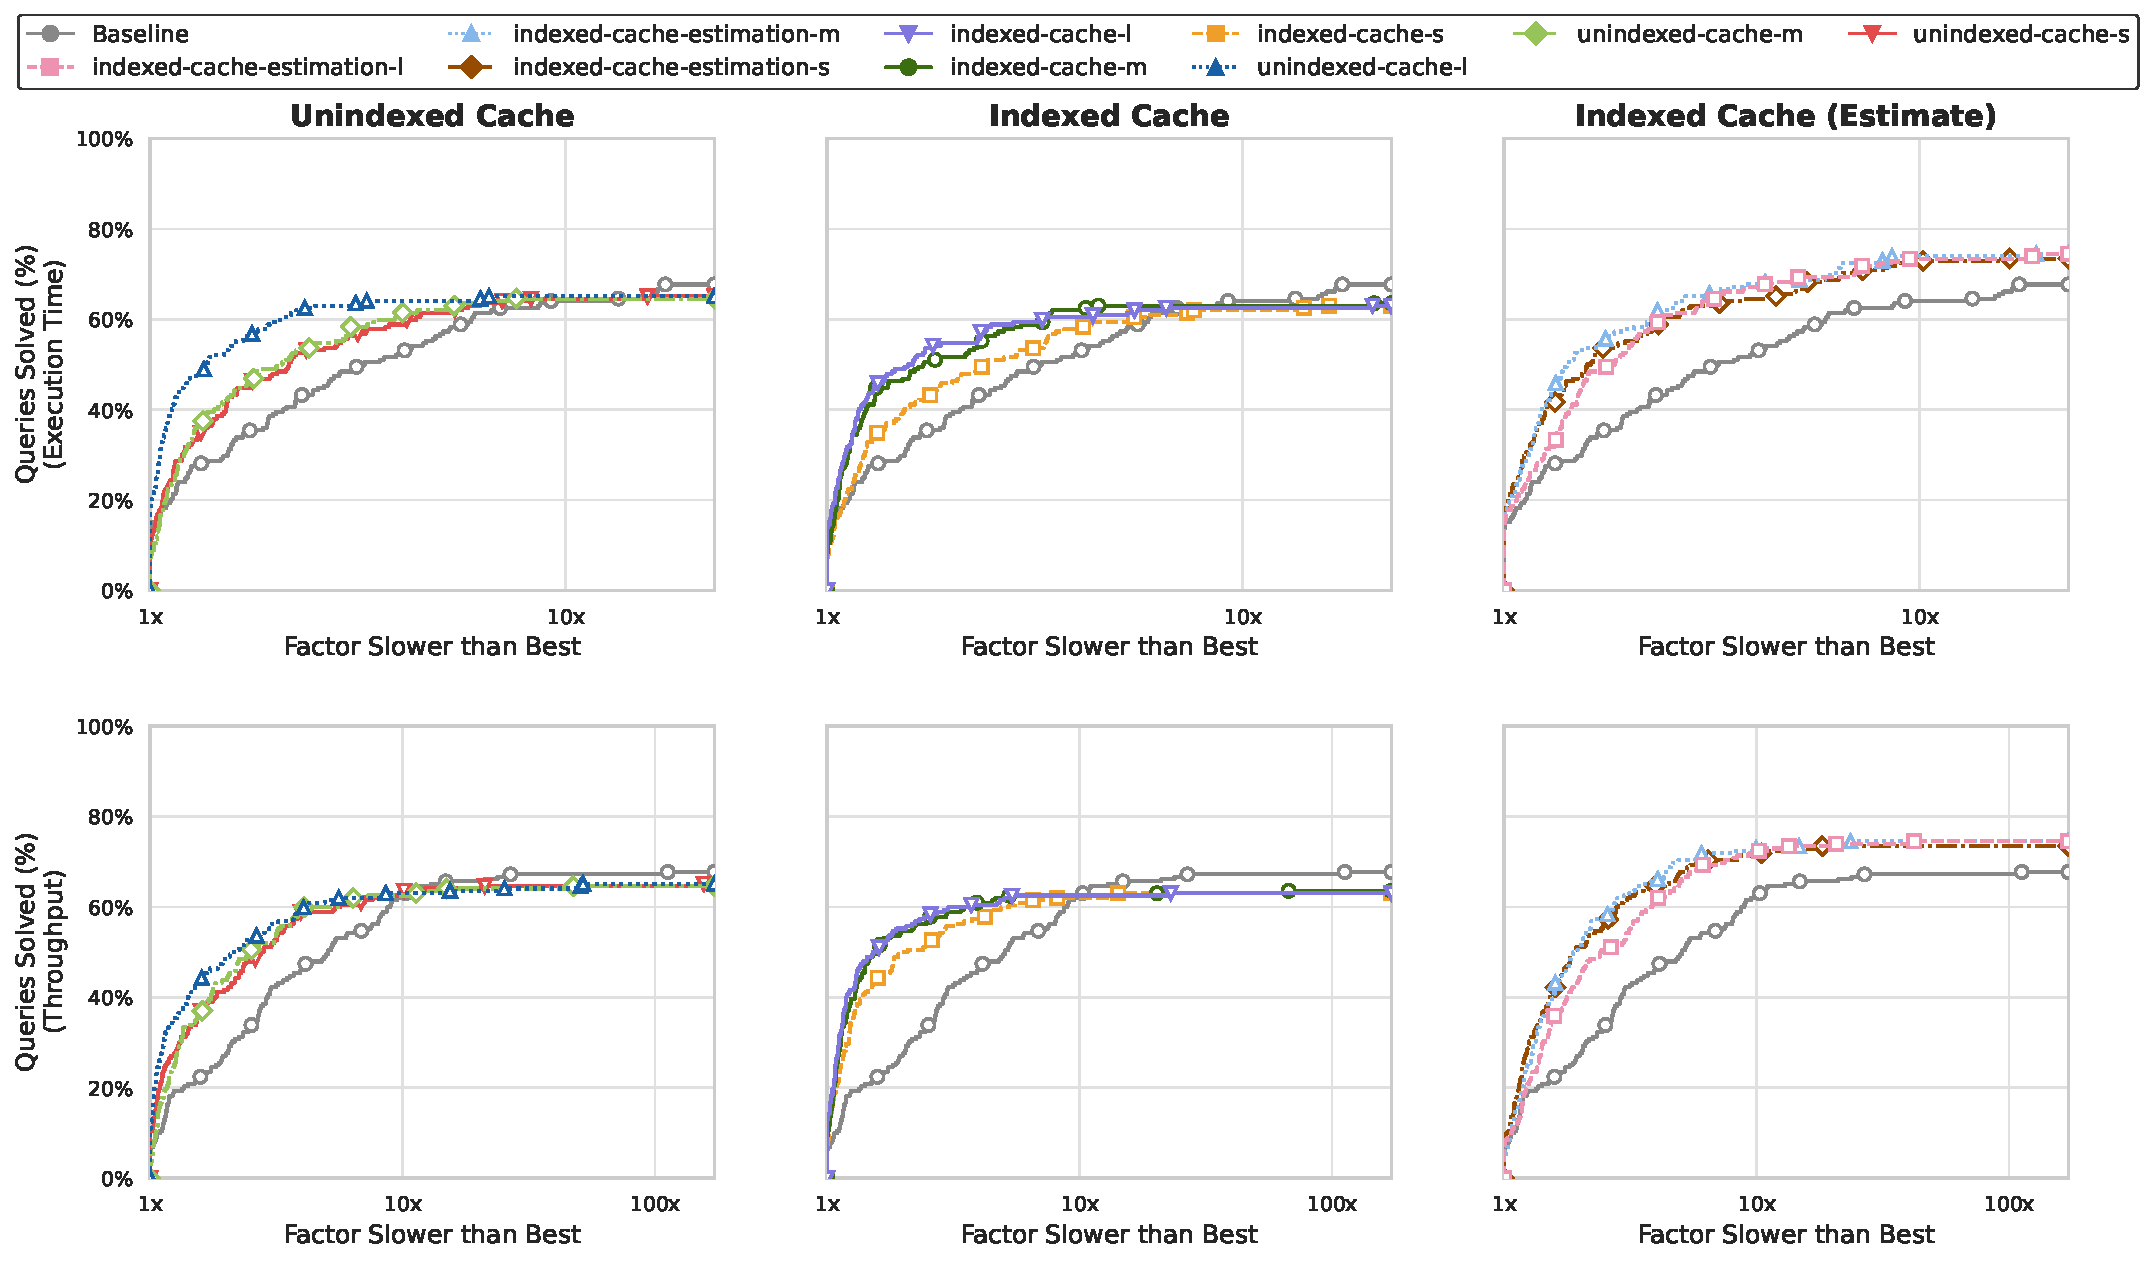
\includegraphics[width=\linewidth]{figures/performance_profile.pdf}
    \caption{Performance profile of caching strategies.
    The x-axis represents the execution time relative to the best-performing algorithm (1x = fastest). 
    The y-axis displays the cumulative percentage of queries successfully resolved within that factor.}
    \label{fig:global_cache_performance}
\end{figure}


\subsection{Logical Sessions}
To evaluate the impact of logical sessions on caching performance, 
we analyze the hit rate deviation ($\Delta$) from the overall average when queries initiate a new session, 
switch to an existing one, or remain in the current session.
Table \ref{tab:performance_differences} shows that new sessions severely degrade hit rates,
existing session switches cause moderate degradation, and intra-session queries improve performance.
These effects are strongest in small and medium caches.

Consequently, optimal client-side cache sizing depends heavily on user session-switching behavior.
These findings highlight the need for eviction policies that better retain cross-session entries
and validate our simulation design;
ignoring session dynamics would obscure critical real-world performance shifts.

Future work should investigate whether query sequences share a frequently accessed core of cache entries.
Protecting these entries from eviction could mitigate the performance penalties of session switching.

\begin{table}[htpb]
\centering
\caption{
    Impact of logical session status on algorithm performance. Values represent absolute and percentage cache hit rate deviations from the global template average across new, existing, and within-session queries.
}
\label{tab:performance_differences}
\begin{tabular*}{\textwidth}{@{\extracolsep{\fill}} l r@{\hspace{1em}}r r@{\hspace{1em}}r r@{\hspace{1em}}r @{}}
\toprule
\textbf{Cache Algorithm} & \multicolumn{2}{c}{\textbf{New Session}} & \multicolumn{2}{c}{\textbf{Existing Session}} & \multicolumn{2}{c}{\textbf{Within Session}} \\
\cmidrule(lr){2-3} \cmidrule(lr){4-5} \cmidrule(lr){6-7}
& \textbf{Abs.} & \textbf{\%} & \textbf{Abs.} & \textbf{\%} & \textbf{Abs.} & \textbf{\%} \\
\midrule
unindexed-l        & -0.066 & -12.278 & -0.014 & -2.474 &  0.011 &  1.931 \\
unindexed-m        & -0.056 & -15.649 & -0.031 & -7.900 &  0.024 &  5.486 \\
unindexed-s        & -0.071 & -24.275 & -0.021 & -6.551 &  0.017 &  4.582 \\
\cmidrule(lr){1-7}
indexed-estimate-l & -0.053 & -10.573 & -0.015 & -2.796 &  0.012 &  2.127 \\
indexed-estimate-m &  0.028 &   7.174 & -0.000 & -0.064 & -0.000 & -0.035 \\
indexed-estimate-s & -0.044 & -14.305 & -0.013 & -3.921 &  0.010 &  2.924 \\
\cmidrule(lr){1-7}
indexed-l          & -0.026 &  -5.011 & -0.003 & -0.571 &  0.003 &  0.467 \\
indexed-m          & -0.087 & -22.782 & -0.021 & -5.098 &  0.017 &  3.682 \\
indexed-s          & -0.033 & -11.036 & -0.015 & -4.470 &  0.012 &  3.153 \\
\bottomrule
\end{tabular*}
\end{table}
\subsection{Refinement Patterns}

To evaluate iterative query refinement simulation, 
we analyze cache behavior across refinement depths. 
Figure 1 shows that hit ratios increase progressively 
as queries undergo sequential refinement. 
Across all algorithms, hit rates increase at depths 2 and 3, 
confirming that refinement heavily reuses prior data.

At higher refinement depths, 
performance depends heavily on cache capacity. 
Large caches sustain high hit rates through depth 4, 
whereas small caches experience significant thrashing,
and degraded hit ratios. 

Surprisingly, the indexed cache without estimation 
maintains high hit rates even with smaller capacities. 
This counterintuitive result stems from implementation differences 
that influence how the single-threaded Node.js event loop 
schedules asynchronous traversal and join executions. 
This scheduling variance alters traversal order and rate, 
ultimately impacting cache eviction and hit performance.


% To evaluate how iterative query development impacts performance, we analyze cache behavior across varying refinement depths.
% Figure 1 demonstrates that cache hit ratios increase progressively as queries undergo sequential modifications from the base template.
% Across all evaluated algorithms, hit rates steadily climb and peak between refinement depths 2 and 3,
% confirming that early exploratory modifications heavily reuse data retrieved by preceding queries.

% However, performance stability at higher refinement depths is highly dependent on cache capacity.
% While large cache configurations successfully sustain high hit rates through depth 4,
% small caches experience significant thrashing at this depth,
% marked by a sharp increase in evictions and a corresponding degradation in the hit ratio.

% Surprisingly, the indexed cache without estimation maintains high hit rates even with smaller cache sizes.
% While these differences might appear counterintuitive, implementation differences directly influence how the single-threaded Node.js event loop schedules asynchronous traversal 
% and join executions. 
% This scheduling variance alters the traversal order and rate, 
% which subsequently impacts cache eviction cycles and overall hit performance.

\begin{figure}[htpb]
    \centering
    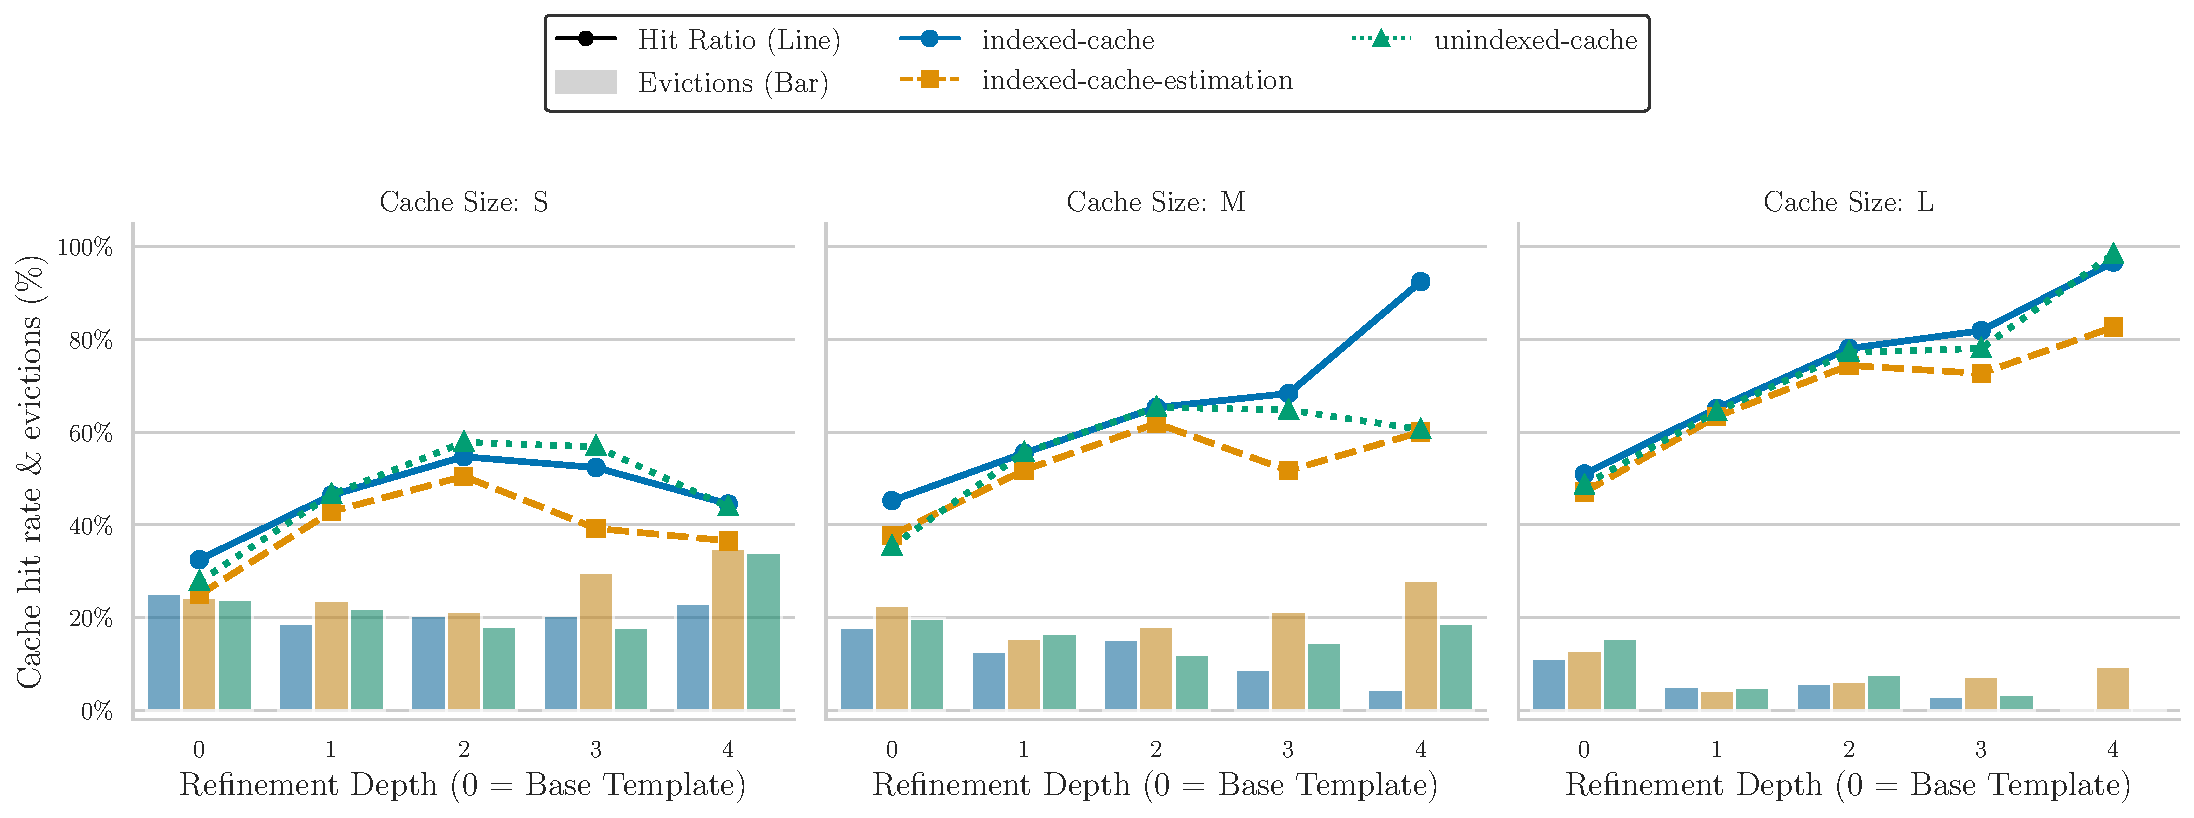
\includegraphics[width=\textwidth]{figures/combined_cache_efficiency.pdf}
    \caption{Cache hit ratios and percentage of cache capacity evicted across refinement depths for small, medium, and large cache configurations.}
    \label{fig:cache_efficiency}
\end{figure}

The observed cache hitrate and eviction differences directly translate to measurable execution speedups.
Figure 2 illustrates that the geometric mean speedup for mainly throughput generally scales positively with refinement depth. 
The indexed-cache algorithm proves particularly effective for prolonged exploratory sequences,
achieving substantial throughput gains at depth 4 compared to the unindexed alternatives.

\begin{figure}[htpb]
    \centering
    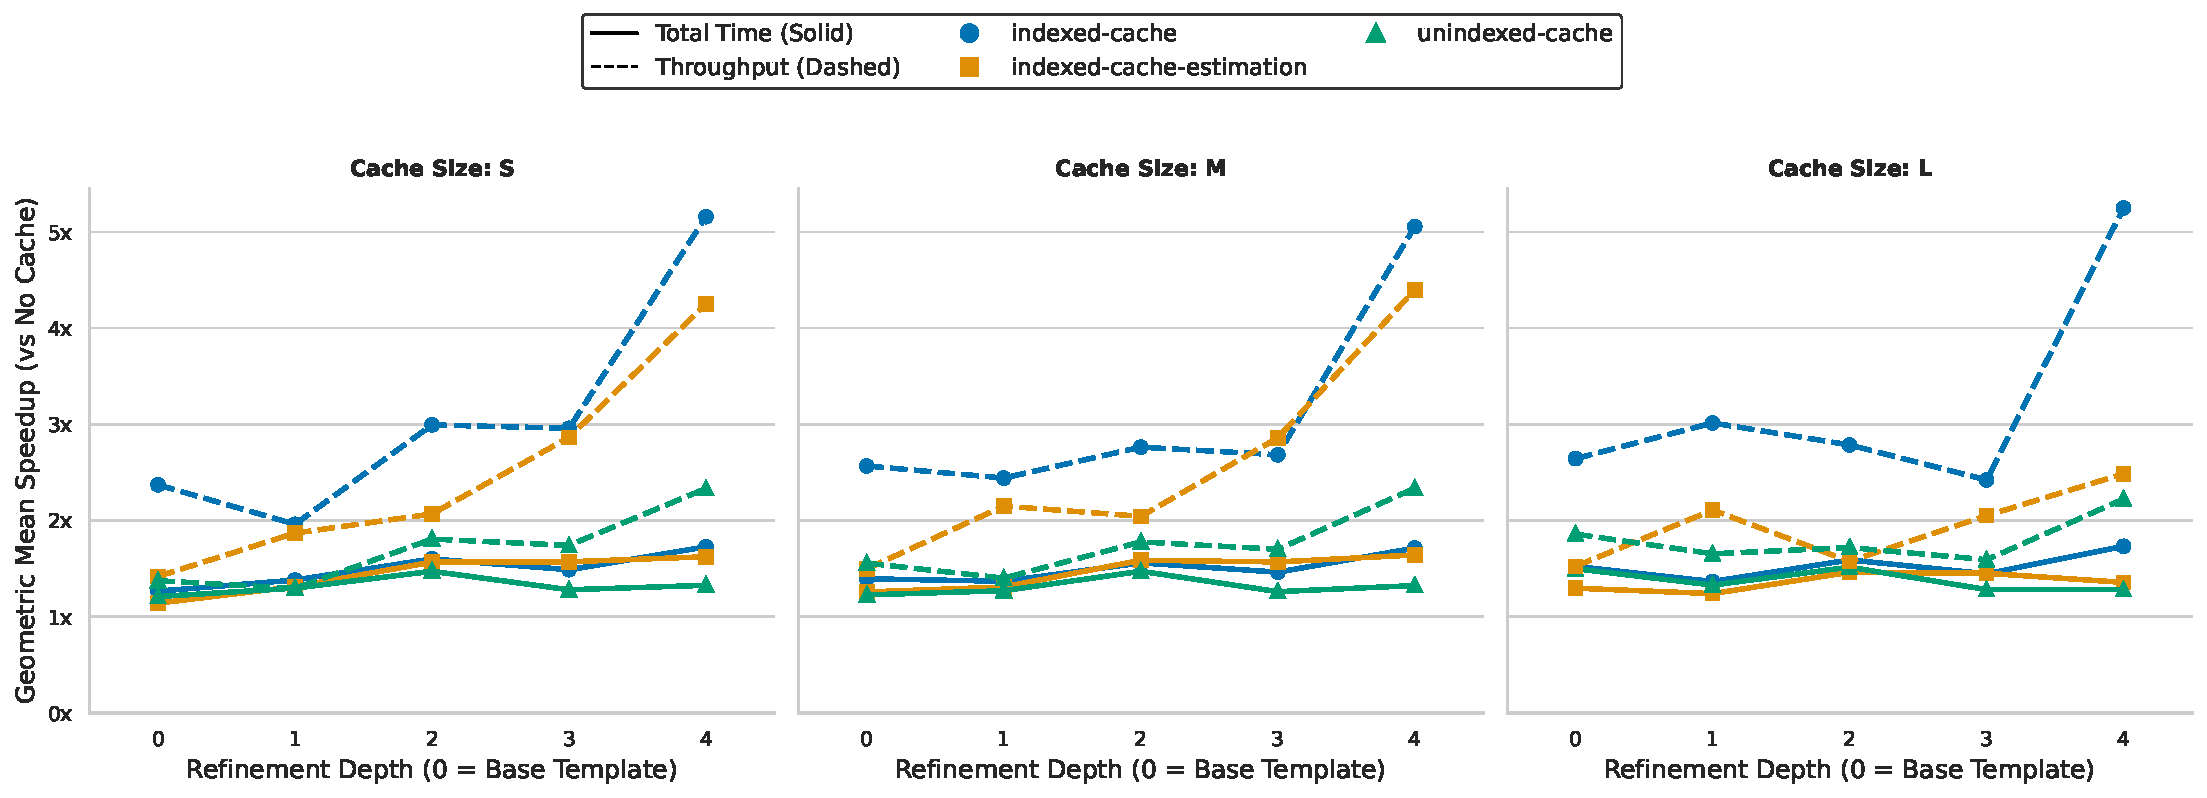
\includegraphics[width=\textwidth]{figures/temporal_throughput_line.pdf}
    \caption{Geometric mean of observed speedups and increases respectively for total execution time and query throughput 
    relative to the no caching baseline across refinement depths.}
    \label{fig:temporal_throughput}
\end{figure}


\subsection{Theoretical Hit Rate Analysis}
To analyze theoretical caching speedup without management costs, we executed one instance of each query template twice 
and simulated cache misses at varying probabilities. 
We excluded the estimation-based approach because using the full cache for estimation would skew the results.

From Figures~\ref{fig:theoretical_cache_performance} and~\ref{fig:theoretical_query_cache_performance}, we find that in most cases caching can significantly improve query execution time, 
with improvements scaling predictably as hit rate increases. 
For some long-running queries such as interactive-discover-6, 7, and short-3 no speedup is observed, with some queries even showing slower result production. 
These query templates traverse many solid pods, but do not require all traversed data. 
In such cases, we hypothesize that having access to a cache which serves documents from memory will quickly produce too much data and slow down result production. 
Thus, waiting for HTTP responses between traversal steps allows the JavaScript event loop to run the join execution pipeline and thus produces results faster as only the first few requests are required for first results.

The two caching approaches exhibit similar overall performance, though the indexed cache significantly reduces the time-to-first-result across most templates. 
As expected, an indexed cache is highly advantageous when in the absence of evictions. 
However, the benchmark results demonstrate that the initial cost of indexing data introduces a clear trade-off:
it amplifies both the potential speedups and slowdowns compared to an unindexed cache.

\begin{figure*}[!h]
    \centering
    % Ensure the filename matches your generated PDF
    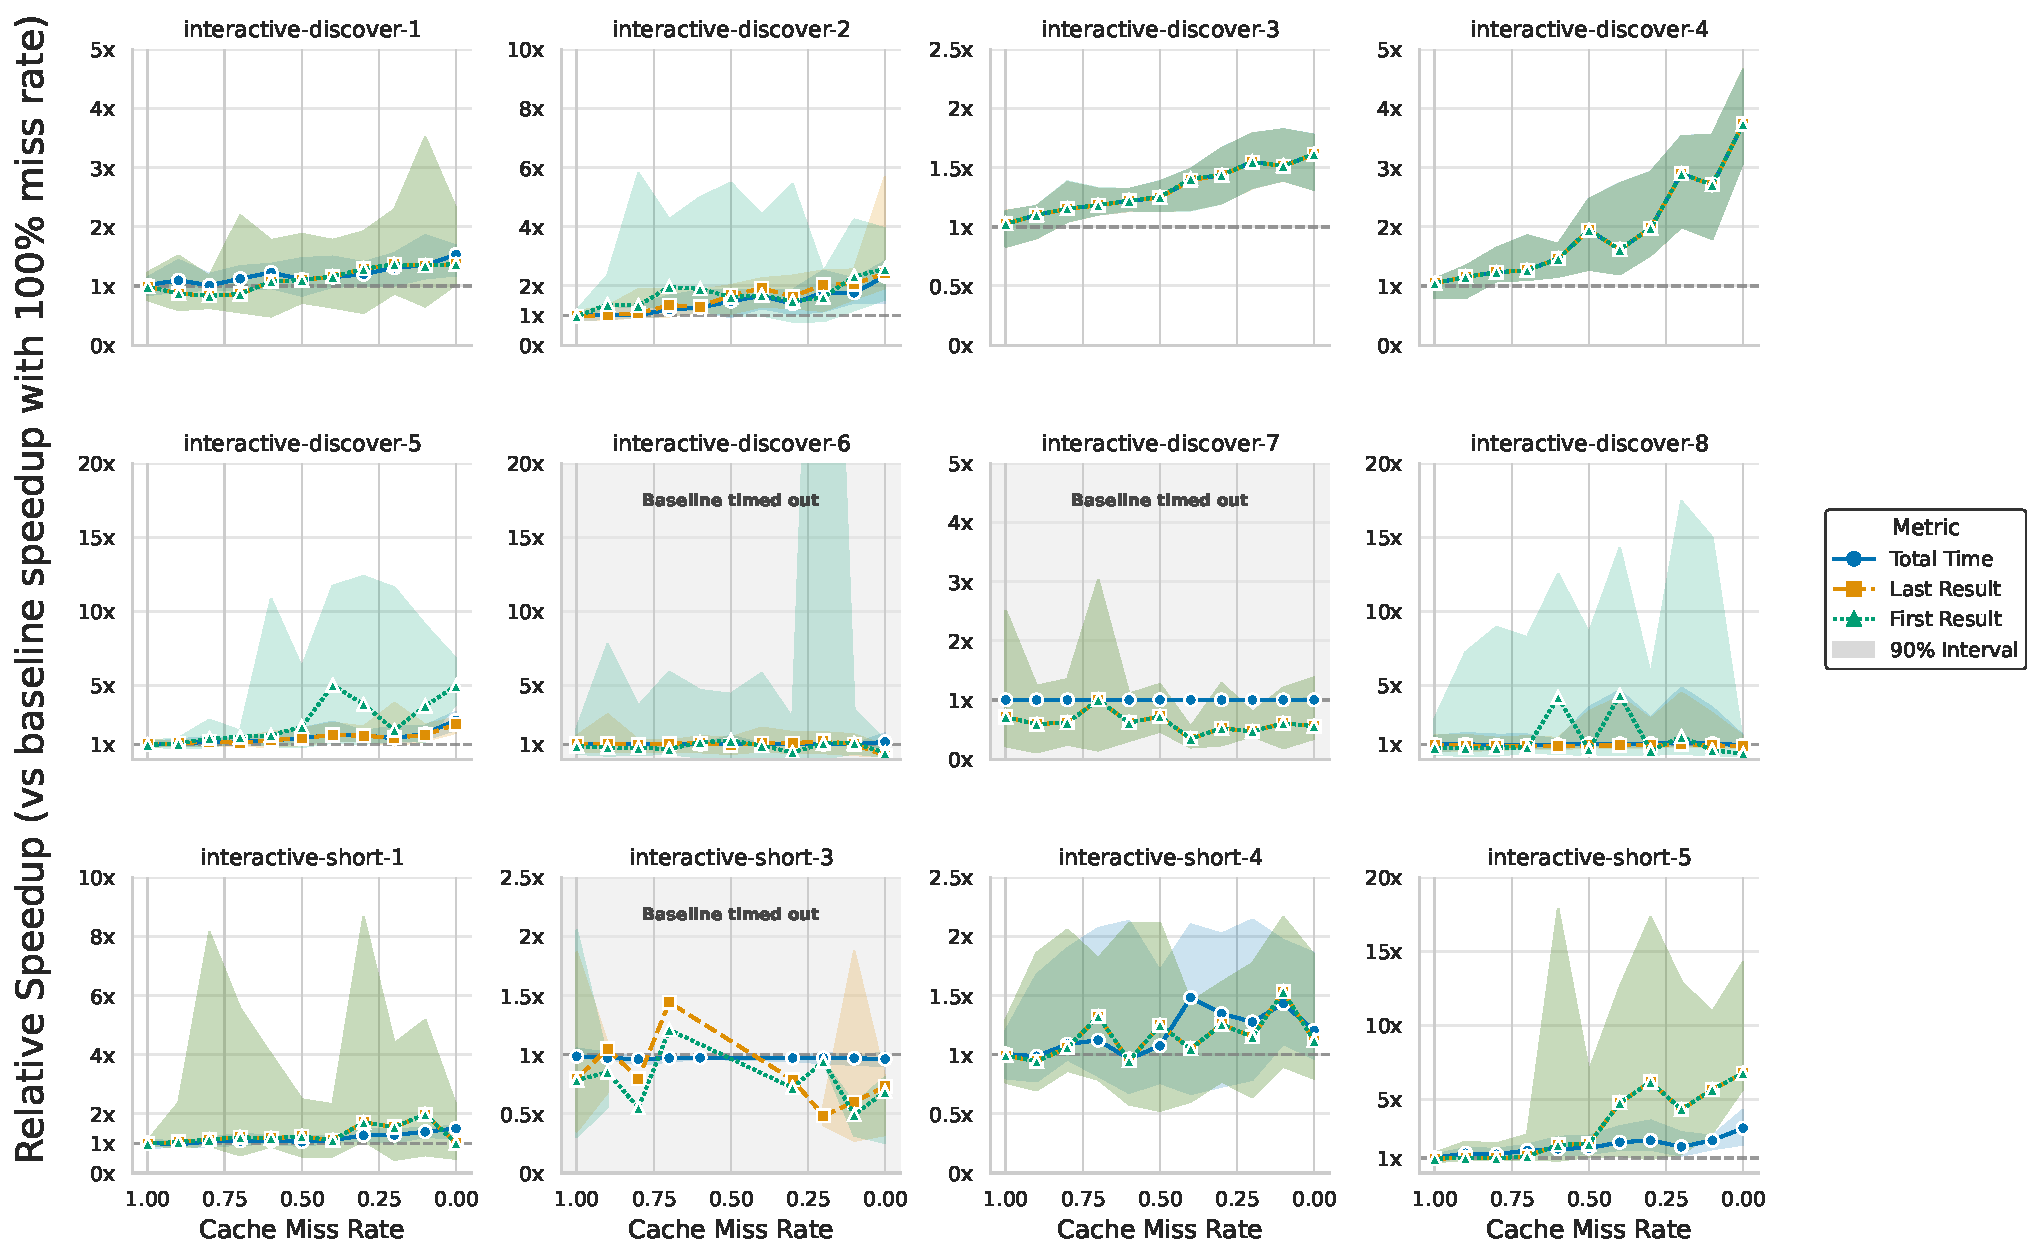
\includegraphics[width=\textwidth]{figures/cache-synth-hitrate.pdf}
    \caption{Theoretical unindexed cache performance by query template. Lines indicate the mean relative speedup of the repeated query for total execution time, first result, and last result against a $100\%$ miss rate baseline. Shaded regions denote the absolute minimum and maximum variance across iterations.}
    \label{fig:theoretical_cache_performance}
\end{figure*}

\begin{figure*}[!h]
    \centering
    % Ensure the filename matches your generated PDF
    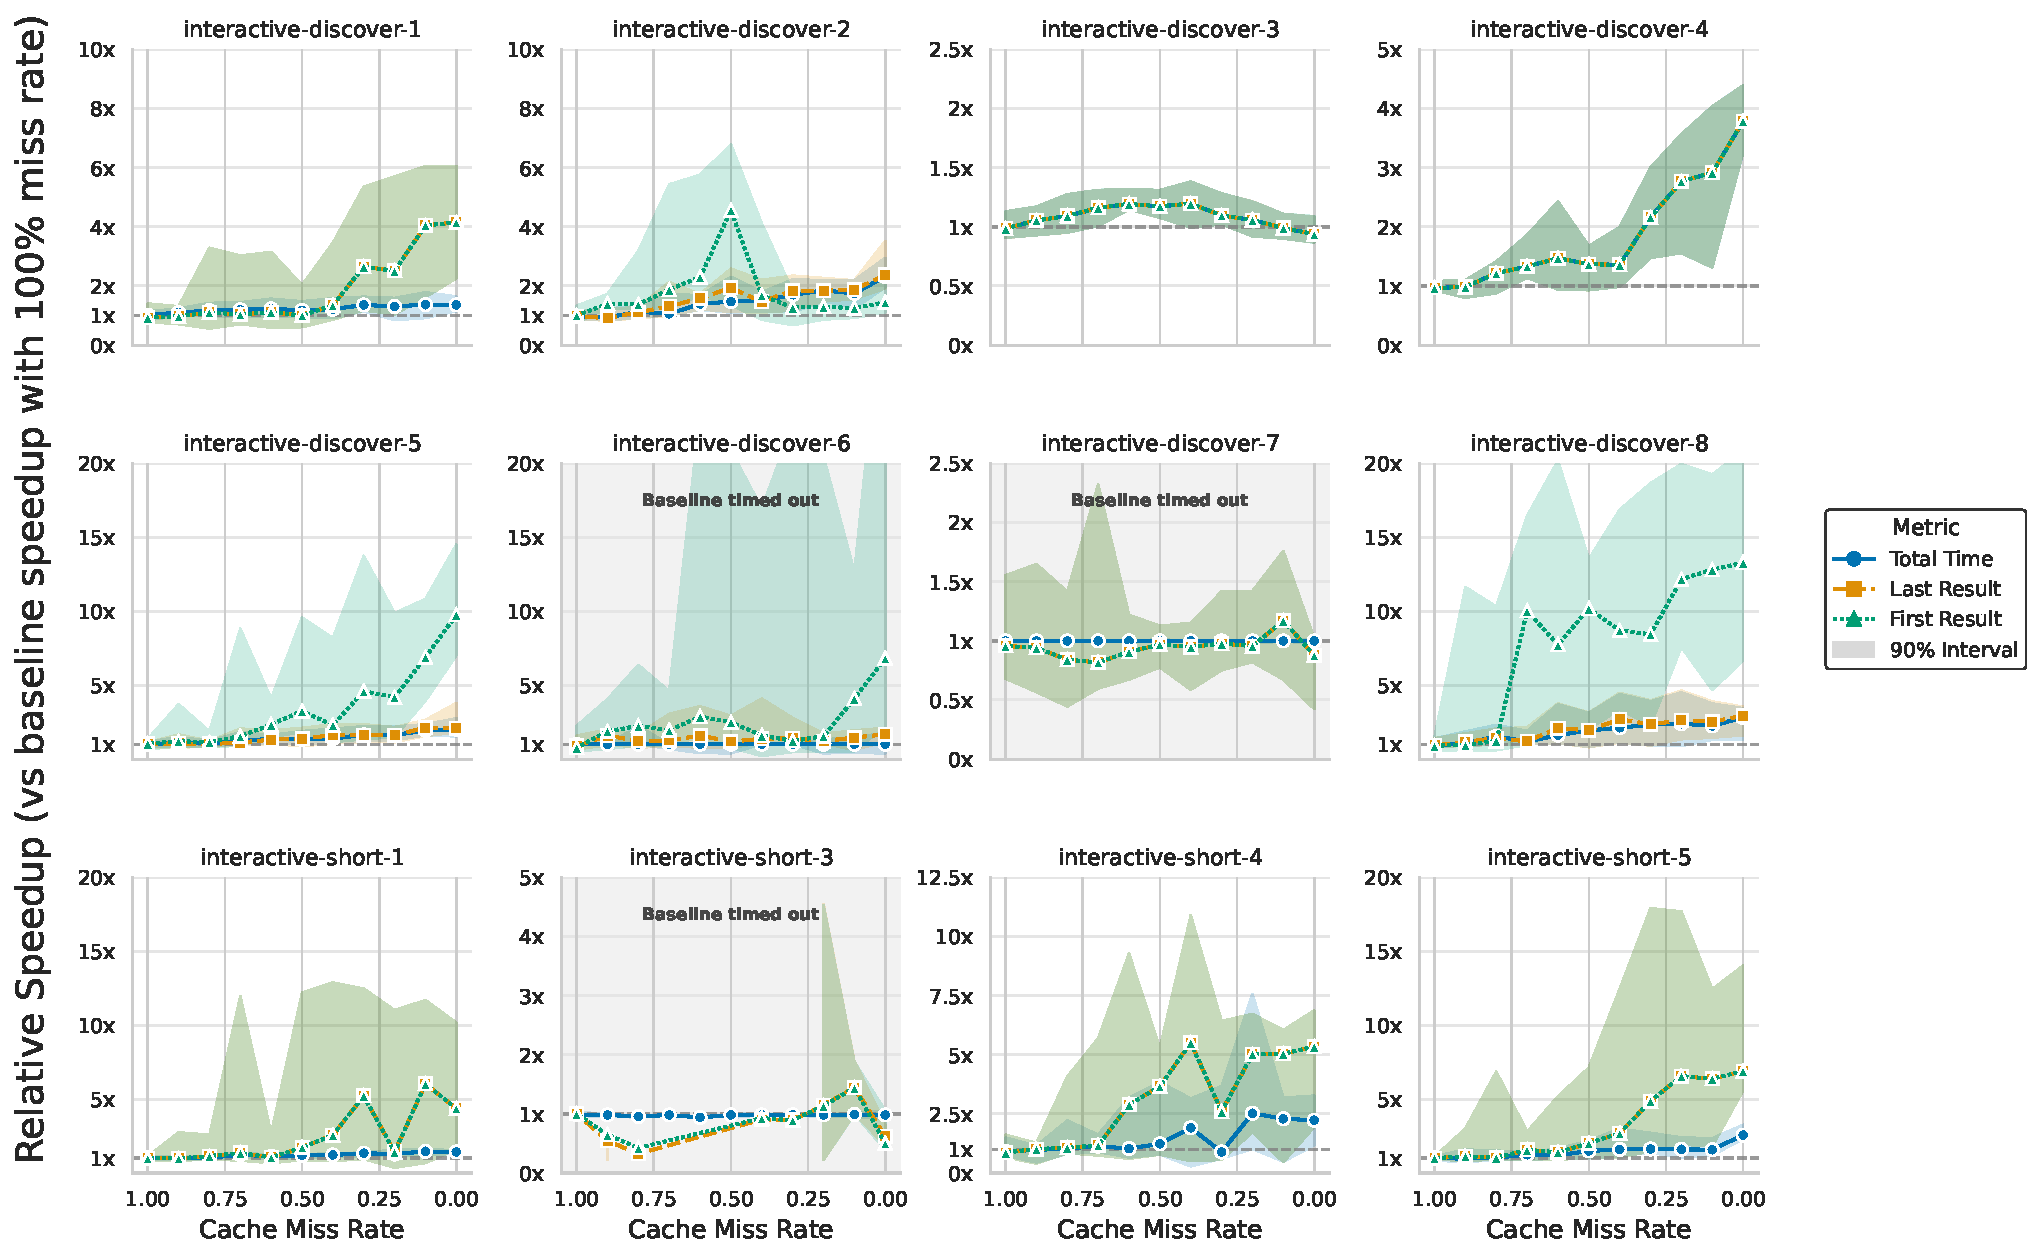
\includegraphics[width=\textwidth]{figures/query-cache-synth-hitrate.pdf}
    \caption{Theoretical indexed cache performance by query template. Lines indicate the mean relative speedup of the repeated query for total execution time, first result, and last result against a $100\%$ miss rate baseline. Shaded regions denote the absolute minimum and maximum variance across iterations.}
    \label{fig:theoretical_query_cache_performance}
\end{figure*}


\subsection{Benchmark Abalations}
